% !TeX root = 场论与凝聚态.tex

The ``microscopic free energy''\footnote{The Mellin transformation of $F$ of variable $\beta$.} will be modified to
\begin{figure}[h]
    \centering
    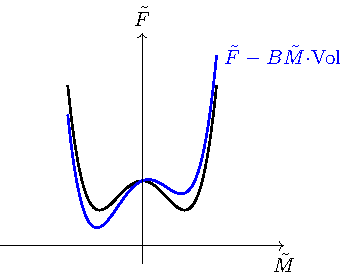
\includegraphics{figures/free_energy_in_external_field.pdf}
    \caption{free energy in external field}
\end{figure}
\begin{equation}
  \tilde{F} = \tilde{F} - B \tilde{M} \cdot \text{Vol}.
\end{equation}
and we have 
\begin{equation}
    \mathcal{Z}\left( B \right)  = \mathrm{e}^{- \frac{F\left( B \right)}{T}} = \int_{-\infty}^{\infty} \mathrm{d}\tilde{M} \, \mathrm{e}^{-\frac{1}{T} \left( \tilde{F} - B \tilde{M} \cdot \text{Vol} \right) } ,
\end{equation}
which is dominated by the double well in $\tilde{F}$.
Meanwhile, we have the relation
\begin{equation}
    M = \frac{1}{\text{Vol}} \frac{\partial F}{\partial B} = \frac{1}{\mathcal{Z}} \frac{\partial \mathcal{Z}}{\partial B} = \left< \tilde{M} \right> 
\end{equation}
and
\begin{equation}
  \chi = \frac{\partial M}{\partial B} = \frac{1}{\mathcal{Z}} \frac{\partial^2 \mathcal{Z}}{\partial B^2} - \frac{1}{\mathcal{Z}^{2}} \frac{\partial \mathcal{Z}}{\partial B} \frac{\partial \mathcal{Z}}{\partial B} = \left< M^{2} \right> - \left< M \right>^{2}
\end{equation}
It can be seen that there's some relation between long range correlation and spontaneous symmetry broken.

\subsection{Long Range Correlation and SSB in Ising Model}

The Hamiltonian of this model is
\begin{equation}
  \begin{gathered}
  H_{\text{classical}} = \sum_{\text{link $l=\langle v\,v' \rangle$}} (-J) \sigma _{v}^{z} \sigma _{v'}^{z}
  \\
  H_{\text{quantum}} = \sum_{\text{vertex $v$}} (-h) \sigma _{v}^{x}+ H_{\text{classical}}
  \end{gathered}
\end{equation}
in which $h$ and $-h$ are equivalent for the $\mathbb{Z}_2$ global symmetry. The corresponding flip operator is
\begin{equation}
  \prod{v} \sigma _{v}^{x}. \quad \text{(one for each part of the space)}
\end{equation}
Note that we doesn't need to flip all spins as our base spacetime may consist separate parts which do not interact with each other.







% TODO 
